\documentclass[12 pt]{article}

%%%%PACKAGE%%%%%%%%%%%%%%%%%%%%%%%%%%%%%%%%%%%%%%%%%%%%%%%%%%%%%%%%%%%%%%%%%%%%
%\usepackage[sfmath]{kpfonts}
\usepackage[latin1]{inputenc} 
\usepackage[T1]{fontenc}      
\usepackage[english,french]{babel}  
\usepackage{amsmath}
%\usepackage{mathtools}
\usepackage{graphicx}
\graphicspath{{images/}}
\usepackage{parskip}
\usepackage{fancyhdr}
\usepackage{layout}
\usepackage{vmargin}
\usepackage{ifthen}
\usepackage[svgnames,dvipsnames]{xcolor}
\graphicspath{{images}}
\usepackage[justification=centering]{caption}
\usepackage{tikz}
\usepackage[linkbordercolor=white]{hyperref}
\usetikzlibrary{fadings}
\usepackage[notmath]{sansmathfonts} %Sans serif pour majuscules textsc
\usepackage{array}
\usepackage{multirow}
\usepackage{svg}
\usepackage{pgfgantt}
\usepackage{titlesec} %espace entre titre et text
%\usepackage{minted} %pour saisir du code

%\usemintedstyle[c++]{default} %style de mise en forme c++
\definecolor{bg}{RGB}{243,230,235} %background color pour le code c++


\usepackage{wasysym} %smiley



\renewcommand{\FrenchLabelItem}{-}
\renewcommand{\subitem}{\newline \quad \textbullet~~  }
\renewcommand{\arraystretch}{1.3}

%%Pour reinitialiser les numeros footnote
\usepackage{perpage} %the perpage package
\MakePerPage{footnote} %the perpage package command
%\usepackage{UPSTI_Pedagogique}\label{key}

\makeatletter
\renewcommand{\thesection}{\@arabic\c@section}
\makeatother


\makeatletter 
\newcommand\mynobreakpar{\par\nobreak\@afterheading} 
\makeatother



\definecolor{HCBleu}{RGB}{26,39,132}
\definecolor{HCBleuclair}{RGB}{148,50,99}

\definecolor{ITEC}{RGB}{218,127,122}
\definecolor{EE}{RGB}{120,229,135}
%\definecolor{SIN}{RGB}{193,214,235}
\definecolor{SIN}{RGB}{162,196,232}
\setlength{\parindent}{1cm} %alinea


\renewcommand\thefootnote{\textbf{\textcolor{HCBleuclair}{\arabic{footnote}}}}

%%%% debut macro couleur legende %%%% 
\makeatletter 
\renewcommand{\fnum@figure}{\textcolor{HCBleuclair}{\normalsize\textbf{\figurename\,\thefigure}}} 

\renewcommand{\fnum@table}{\textcolor{HCBleuclair}{\textsc{\textbf{Tableau\,\thetable}}}}

\makeatother 


%%%% fin macro couleur legende %%%%


\newcommand{\gradient}[1]{\noindent%
	\begin{tikzpicture}
	\fill[left color=HCBleu,right color=HCBleuclair] rectangle (\linewidth,0.16cm);
	\node at (0.5\linewidth,0.05) {\bfseries #1};
	%\fill[cyan,path fading=west] (0,-1em) rectangle (\linewidth,-1.5em);
	\end{tikzpicture}%
}

\newcommand{\ligneg}[1]{\noindent%
	\begin{tikzpicture}
	
	\fill[left color=HCBleu,right color=HCBleuclair] rectangle (\linewidth,0.07cm);
	\node at (.5\linewidth,0.05) {\bfseries #1};
	%\fill[cyan,path fading=west] (0,-1em) rectangle (\linewidth,-1.5em);
	\end{tikzpicture}%
}

\newcommand{\lignegg}[1]{\noindent%
	\begin{tikzpicture}
	
	\fill[left color=HCBleu,right color=HCBleuclair] rectangle (\linewidth,0.07cm);
	\node at (.5\linewidth,0.5) {\bfseries #1};
	%\fill[cyan,path fading=west] (0,-1em) rectangle (\linewidth,-1.5em);
	\end{tikzpicture}%
}

\renewcommand\familydefault{\sfdefault}  %police sans serif

\usepackage{setspace} % pour gerer l'interligne (je crois)


%%%%MARGE%%%%%%%%%%%%%%%%%%%%%%%%%%%%%%%%%%%%%%%%%%%%%%%%%%%%%%%%%%%%%%%%%%%%%%
\setmarginsrb{2.5 cm}{1cm}{2.5 cm}{1.5 cm}{0.3 cm}{0.2 cm}{0 cm}{0 cm}
%1 est la marge gauche
%2 est la marge en haut
%3 est la marge droite
%4 est la marge en bas
%5 fixe la hauteur de l'entete
%6 fixe la distance entre l'entete et le texte
%7 fixe la hauteur du pied de page
%8 fixe la distance entre le texte et le pied de page
\pagestyle{fancy}

%%%%En-tête et pied de page POUR LA VERSION A IMPRIMER  %%%%%%%%%%%%%%%%%%%%%%%

\renewcommand\headrule{\ligneg{}}
\fancyhead[R]{}
\fancyhead[L]{}
%\fancyhead[RE]{\nouppercase{\textbf{\leftmark}}}
%\fancyhead[RO]{\textbf{\thepage}} 


%\renewcommand\footrulewidth{1pt}

\fancyfoot[C]{}
%\fancyfoot[R]{Session 2020}
%\fancyfoot[L]{Agrégation SII - Option IM}

%%%%%%%%%%%%%%%%%%%%%%%%%%%%%%%%%%%%%%%%%%%%%%%%%%%%%%%%%%%%%%%%%%%%%%%%%%%%%%%
%%%%En-tete et pied de page POUR LA VERSION NUMERIQUE  %%%%%%%%%%%%%%%%%%%%%%%%

%%%%A FAIRE, 
%%attention, j'ai mis le parametre twoside dans le document class

%%%%%%%%%%%%%%%%%%%%%%%%%%%%%%%%%%%%%%%%%%%%%%%%%%%%%%%%%%%%%%%%%%%%%%%%%%%%%%%
%%%%%%%%%%%%%%%%%%%%%%%%%%DOCUMENT%%%%%%%%%%%%%%%%%%%%%%%%%%%%%%%%%%%%%%%%%%%%%

\newcommand\vect[1]{\overrightarrow{#1}}

\newcolumntype{M}[1]{>{\centering\arraybackslash}m{#1}}
\newcolumntype{P}[1]{>{\raggedright\arraybackslash}p{#1}}

\setlength\abovecaptionskip{0.2cm} %espace entre legende et figure
\setlength\belowcaptionskip{-0.2cm} %espace entre legende et paragraphe


\titlespacing*{\section}
{0pt}{4ex}{1.8ex}
\titlespacing*{\subsection}
{0pt}{2.1ex}{1.8ex}
\titlespacing*{\subsubsection}
{0pt}{1.8ex}{1.6ex}
\titlespacing*{\paragraph}
{0pt}{1.8ex}{1.8ex}



\usepackage{afterpage} %Pour le compteur de page
\newcommand\myemptypage{
	\newpage
	\null
	\thispagestyle{empty}
	\addtocounter{page}{-1}
	\newpage	
}


\begin{document}
\begin{center}
	\vspace*{-0.3cm}
	{\Large \textbf{Deep learning for hand prosthesis piloting based on sEMG signals\\}}
	\vspace{0.5cm}
	{\large Project proposal \\}
	\vspace{0.3cm}
	{\large\textbf{Antoine Benady, Raphael Reme} \\}
	\vspace{0.3cm}
	%{29 october 2020\\}
	%\vspace{2cm}
	\lignegg{}
\end{center}

% \begin{center}
% 	\small{\textit{Si t'es chaud pour bosser avec moi sur ce projet \smiley}
% 		%\vspace{1cm}
% 	}
% \end{center}


\section*{Context}
Active, handy and cheap hand prosthesis conception is currently a challenge. It's limited by the complexity of the movements of the human hands, and by
the interpretation of the user's will.

The problem is often stated as a classification problem \cite{classification}, where the goal is to find the movement desired
by the user among a set of gestures and then execute it. But this formulation of the problem is really limited by the number of
gestures considered, and does not grant an intuitive control over the prosthesis. Some recent results seem to show that, with the recent breakthroughs
in deep learning, the regression problem could be adressed. (Guessing directly all the relative positions of the hand from the user's will.)
It brings a much more intuitive control over the prosthesis and is not limited by a set of pre-defined gestures.

The question is on which data can be based the user's will extraction ? One of the cheaper approach is to rely only on surface electromyography
(sEMG) signals acquired from the forearm muscles. These signals are cheap to extract but hard to exploit in order to predict the hand movements.

Our goal will be to use Recurrent Neural Networks (RNNs) in order to exploit the temporal dependencies of sEMG and predict the positions of the hand.


\begin{figure}[!htbp]
	\centering
	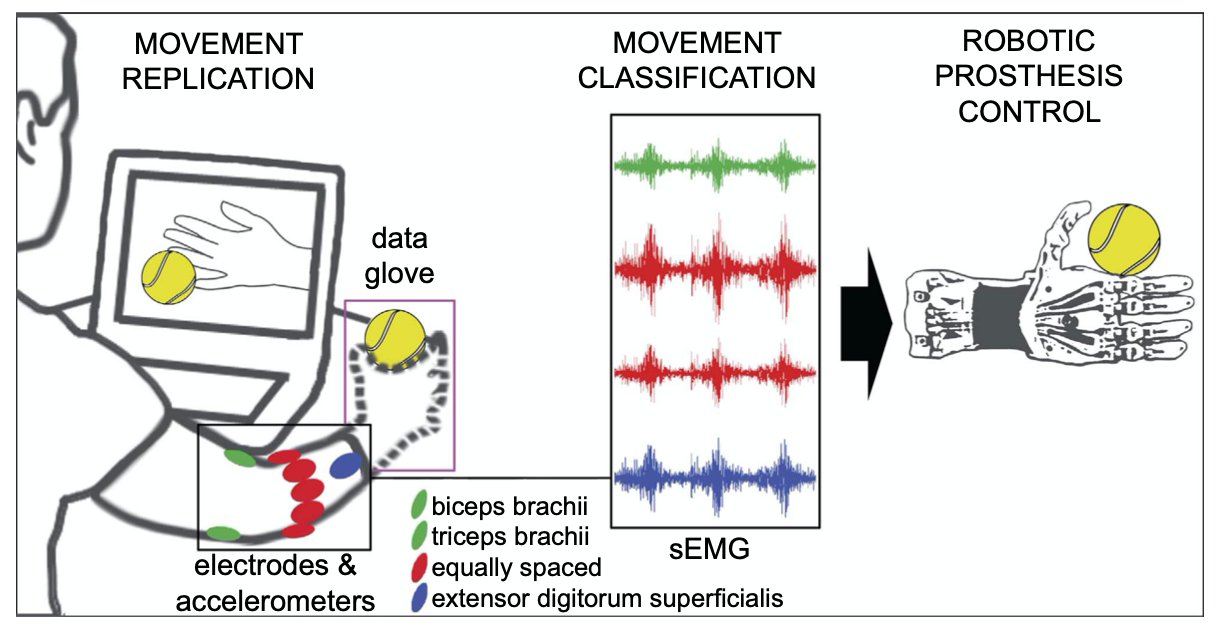
\includegraphics[width=14cm]{plan}
	\caption{Prosthesis control from sEMG and a gesture classification processus. \cite{principe}}
\end{figure}

\section*{Methodology}
A review of the literature found that RNN-based approaches are promising for solving the regression problem \cite{Koch}.
In this project, we would like to implement RNNS to solve it. A reasonable objective is to reach the same performance found in the literature.

Our methodology is the following :
\begin{itemize}
	\item Extract a dataset relevant to the problem such as one (or several) Ninapro database(s) \cite{database}.
	\item Implement a recurrent neural networks with the use of LSTM cells (Long-short terms memory). We plan to test several architecture to reach the
	      best performance.
	\item Validate our results with the evaluation method detailled in the following section.
\end{itemize}

\section*{Evaluation}
The Ninapro Database \cite{database} is one of the most commonly used database in the field. It records sEMG and the general position of the hand
(resumed by 22 positions of sensors placed on it) during the realisation of some specific gesture. It can therefore be used both for classification,
where the goal find the gesture, and regression, where you guess the positions of the hand.

Our objective is to create and learn a network able to predict the positions of the 22 glove's sensors for each time t knowing the sEMG signals of the
previous times. The database will provides us the 22 positions at each time, allowing us to train and evaluate a RNN model.

It could also be nice to modelise in 3D the hand from the 22 positions and therefore to show some results on a 3D model. The point would be to
see the impact of the errors on the reconstructed hand.

\bibliographystyle{plain}
\bibliography{biblio}


\end{document}
